\documentclass[12pt,twoside]{article}
\usepackage[dvipsnames]{xcolor}
\usepackage{tikz,graphicx,amsmath,amsfonts,amscd,amssymb,bm,cite,epsfig,epsf,url}
\usepackage[hang,flushmargin]{footmisc}
\usepackage[colorlinks=true,urlcolor=blue,citecolor=blue]{hyperref}
\usepackage{amsthm,multirow,wasysym,appendix}
\usepackage{array,subcaption} 
% \usepackage[small,bf]{caption}
\usepackage{bbm}
\usepackage{pgfplots}
\usetikzlibrary{spy}
\usepgfplotslibrary{external}
\usepgfplotslibrary{fillbetween}
\usetikzlibrary{arrows,automata}
\usepackage{thmtools}
\usepackage{blkarray} 
\usepackage{textcomp}
\usepackage[left=0.8in,right=1.0in,top=1.0in,bottom=1.0in]{geometry}
\usepackage{pifont}
\usepackage{tikz-qtree}

%% Probability operators and functions
%
% \def \P{\mathrm{P}}
\def \P{\mathrm{P}}
\def \E{\mathrm{E}}
\def \Var{\mathrm{Var}}
\let\var\Var
\def \Cov {\mathrm{Cov}} \let\cov\Cov
\def \MSE {\mathrm{MSE}} \let\mse\MSE
\def \sgn {\mathrm{sgn}}
\def \R {\mathbb{R}}
\def \C {\mathbb{C}}
\def \N {\mathbb{N}}
\def \Z {\mathbb{Z}}
\def \cV {\mathcal{V}}
\def \cS {\mathcal{S}}

\newcommand{\RR}{\ensuremath{\mathbb{R}}}

\DeclareMathOperator*{\argmin}{arg\,min}
\DeclareMathOperator*{\argmax}{arg\,max}
\newcommand{\red}[1]{\textcolor{red}{#1}}
\newcommand{\blue}[1]{\textcolor{blue}{#1}}
\newcommand{\green}[1]{\textcolor{ForestGreen}{ #1}}
\newcommand{\fuchsia}[1]{\textcolor{RoyalPurple}{ #1}}



%
%% Probability distributions
%
%\def \Bern    {\mathrm{Bern}}
%\def \Binom   {\mathrm{Binom}}
%\def \Exp     {\mathrm{Exp}}
%\def \Geom    {\mathrm{Geom}}
% \def \Norm    {\mathcal{N}}
%\def \Poisson {\mathrm{Poisson}}
%\def \Unif    {\mathrm {U}}
%
\DeclareMathOperator{\Norm}{\mathcal{N}}

\newcommand{\bdb}[1]{\textcolor{red}{#1}}

\newcommand{\ml}[1]{\mathcal{ #1 } }
\newcommand{\wh}[1]{\widehat{ #1 } }
\newcommand{\wt}[1]{\widetilde{ #1 } }
\newcommand{\conj}[1]{\overline{ #1 } }
\newcommand{\rnd}[1]{\tilde{ #1 } }
\newcommand{\rv}[1]{ \rnd{ #1}  }
\newcommand{\rM}{\rnd{ m}  }
\newcommand{\rx}{\rnd{ x}  }
\newcommand{\ry}{\rnd{ y}  }
\newcommand{\rz}{\rnd{ z}  }
\newcommand{\ra}{\rnd{ a}  }
\newcommand{\rb}{\rnd{ b}  }
\newcommand{\rt}{\rnd{ t}  }
\newcommand{\rs}{\rnd{ s}  }


\newcommand{\rpc}{\widetilde{ pc}  }
\newcommand{\rndvec}[1]{\vec{\rnd{#1}}}

\def \cnd {\, | \,}
\def \Id { I }
\def \J {\mathbf{1}\mathbf{1}^T}

\newcommand{\op}[1]{\operatorname{#1}}
\newcommand{\setdef}[2]{ := \keys{ #1 \; | \; #2 } }
\newcommand{\set}[2]{ \keys{ #1 \; | \; #2 } }
\newcommand{\sign}[1]{\op{sign}\left( #1 \right) }
\newcommand{\trace}[1]{\op{tr}\left( #1 \right) }
\newcommand{\tr}[1]{\op{tr}\left( #1 \right) }
\newcommand{\inv}[1]{\left( #1 \right)^{-1} }
\newcommand{\abs}[1]{\left| #1 \right|}
\newcommand{\sabs}[1]{| #1 |}
\newcommand{\keys}[1]{\left\{ #1 \right\}}
\newcommand{\sqbr}[1]{\left[ #1 \right]}
\newcommand{\sbrac}[1]{ ( #1 ) }
\newcommand{\brac}[1]{\left( #1 \right) }
\newcommand{\bbrac}[1]{\big( #1 \big) }
\newcommand{\Bbrac}[1]{\Big( #1 \Big)}
\newcommand{\BBbrac}[1]{\BIG( #1 \Big)}
\newcommand{\MAT}[1]{\begin{bmatrix} #1 \end{bmatrix}}
\newcommand{\sMAT}[1]{\left(\begin{smallmatrix} #1 \end{smallmatrix}\right)}
\newcommand{\sMATn}[1]{\begin{smallmatrix} #1 \end{smallmatrix}}
\newcommand{\PROD}[2]{\left \langle #1, #2\right \rangle}
\newcommand{\PRODs}[2]{\langle #1, #2 \rangle}
\newcommand{\der}[2]{\frac{\text{d}#2}{\text{d}#1}}
\newcommand{\pder}[2]{\frac{\partial#2}{\partial#1}}
\newcommand{\derTwo}[2]{\frac{\text{d}^2#2}{\text{d}#1^2}}
\newcommand{\ceil}[1]{\lceil #1 \rceil}
\newcommand{\Imag}[1]{\op{Im}\brac{ #1 }}
\newcommand{\Real}[1]{\op{Re}\brac{ #1 }}
\newcommand{\norm}[1]{\left|\left| #1 \right|\right| }
\newcommand{\norms}[1]{ \| #1 \|  }
\newcommand{\normProd}[1]{\left|\left| #1 \right|\right| _{\PROD{\cdot}{\cdot}} }
\newcommand{\normTwo}[1]{\left|\left| #1 \right|\right| _{2} }
\newcommand{\normTwos}[1]{ \| #1  \| _{2} }
\newcommand{\normZero}[1]{\left|\left| #1 \right|\right| _{0} }
\newcommand{\normTV}[1]{\left|\left| #1 \right|\right|  _{ \op{TV}  } }% _{\op{c} \ell_1} }
\newcommand{\normOne}[1]{\left|\left| #1 \right|\right| _{1} }
\newcommand{\normOnes}[1]{\| #1 \| _{1} }
\newcommand{\normOneTwo}[1]{\left|\left| #1 \right|\right| _{1,2} }
\newcommand{\normF}[1]{\left|\left| #1 \right|\right| _{\op{F}} }
\newcommand{\normLTwo}[1]{\left|\left| #1 \right|\right| _{\ml{L}_2} }
\newcommand{\normNuc}[1]{\left|\left| #1 \right|\right| _{\ast} }
\newcommand{\normOp}[1]{\left|\left| #1 \right|\right|  }
\newcommand{\normInf}[1]{\left|\left| #1 \right|\right| _{\infty}  }
\newcommand{\proj}[1]{\mathcal{P}_{#1} \, }
\newcommand{\diff}[1]{ \, \text{d}#1 }
\newcommand{\vc}[1]{\boldsymbol{\vec{#1}}}
\newcommand{\rc}[1]{\boldsymbol{#1}}
\newcommand{\vx}{\vec{x}}
\newcommand{\vy}{\vec{y}}
\newcommand{\vz}{\vec{z}}
\newcommand{\vu}{\vec{u}}
\newcommand{\vv}{\vec{v}}
\newcommand{\vb}{\vec{\beta}}
\newcommand{\va}{\vec{\alpha}}
\newcommand{\vaa}{\vec{a}}
\newcommand{\vbb}{\vec{b}}
\newcommand{\vg}{\vec{g}}
\newcommand{\vw}{\vec{w}}
\newcommand{\vh}{\vec{h}}
\newcommand{\vbeta}{\vec{\beta}}
\newcommand{\valpha}{\vec{\alpha}}
\newcommand{\vgamma}{\vec{\gamma}}
\newcommand{\veta}{\vec{\eta}}
\newcommand{\vnu}{\vec{\nu}}
\newcommand{\rw}{\rnd{w}}
\newcommand{\rvnu}{\vc{\nu}}
\newcommand{\rvv}{\rndvec{v}}
\newcommand{\rvw}{\rndvec{w}}
\newcommand{\rvx}{\rndvec{x}}
\newcommand{\rvy}{\rndvec{y}}
\newcommand{\rvz}{\rndvec{z}}
\newcommand{\rvX}{\rndvec{X}}


\newtheorem{theorem}{Theorem}[section]
% \declaretheorem[style=plain,qed=$\square$]{theorem}
\newtheorem{corollary}[theorem]{Corollary}
\newtheorem{definition}[theorem]{Definition}
\newtheorem{lemma}[theorem]{Lemma}
\newtheorem{remark}[theorem]{Remark}
\newtheorem{algorithm}[theorem]{Algorithm}

% \theoremstyle{definition}
%\newtheorem{example}[proof]{Example}
\declaretheorem[style=definition,qed=$\triangle$,sibling=definition]{example}
\declaretheorem[style=definition,qed=$\bigcirc$,sibling=definition]{application}

%
%% Typographic tweaks and miscellaneous
%\newcommand{\sfrac}[2]{\mbox{\small$\displaystyle\frac{#1}{#2}$}}
%\newcommand{\suchthat}{\kern0.1em{:}\kern0.3em}
%\newcommand{\qqquad}{\kern3em}
%\newcommand{\cond}{\,|\,}
%\def\Matlab{\textsc{Matlab}}
%\newcommand{\displayskip}[1]{\abovedisplayskip #1\belowdisplayskip #1}
%\newcommand{\term}[1]{\emph{#1}}
%\renewcommand{\implies}{\;\Rightarrow\;}



\begin{document}

\begin{center}
{\large{\textbf{Homework 11}} } \vspace{0.2cm}\\
Due April 23 at 11 pm
\\
\end{center}
Unless stated otherwise, justify any answers you give.
You can work in groups, but each
student must write their own solution based on their own
understanding of the problem.

When uploading your homework to Gradescope you will have to
select the relevant pages for each question.  Please submit each
problem on a separate page (i.e., 1a and~1b can be on the same page but 1
and 2 must be on different pages).  We understand that this may be
cumbersome but this is the best way for the grading team to grade your
homework assignments and provide feedback in a timely manner.  Failure
to adhere to these guidelines may result in a loss of points.
Note that it may take some time to
select the pages for your submission.  Please plan accordingly.  We
suggest uploading your assignment at least 30 minutes before the deadline
so you will have ample time to select the correct pages for your
submission.  If you are using \LaTeX, consider using the minted or
listings packages for typesetting code.  
\\

\begin{enumerate}

 \item (Heartbeat) We are interested estimating the heartbeat of a fetus in the presence of strong interference in the form of the heartbeat of the baby's mother. To simplify matters, let us assume that we only want to estimate the heartbeat at a certain moment. We acquire data using a microphone situated near the mother's belly and also a microphone that is away from her belly. We model the data as
\begin{align}
\rx[1] & = \rb + \rnd{m} + \rnd{z}_1\\
\rx[2] & = \rnd{m} + \rnd{z}_2,
\end{align}
where $\rb$ is a random variable modeling the heartbeat of the baby, $\rnd{m}$ is a random variable modeling the heartbeat of the mother, and $\rnd{z}_1$ and $\rnd{z}_2$ model additive noise. All random variables are centered to have zero mean. From past data, we determine that $\rb$, $\rnd{m}$, $\rnd{z}_1$, and $\rnd{z}_2$ are all uncorrelated with each other. The variances of $\rb$, $\rnd{z}_1$ and $\rnd{z}_2$ are equal to $1$, whereas the variance of $\rnd{m}$ is much larger, it is equal to $10$.
\begin{enumerate}
\item Compute the linear MMSE of $\rb$ given $\rx[1]$, and the corresponding coefficient of determination.  
\begin{itemize}
    \color{blue}
    \item so we our linear model in this case would be $$\ell(\Tilde{x}_1)=\beta \Tilde{x}_1 + \alpha$$ for some coefficients $\alpha, \beta$
    \item first lets look at the best constant estimator in terms of mean squared error 
    \begin{itemize}
        \item we can write $$\ell(c)=E[(\Tilde{y}- c)^2]=E[\Tilde{y}^2 - 2c\Tilde{y}+c^2]= E[\Tilde{y}^2] - 2cE[\Tilde{y}]-c^2$$
        \item and we can see $$\nabla \ell(c)=-2E[\Tilde{y}]+2c$$ and $$\nabla \ell(c)'=2$$ and thus function is convex meaning we have a global optima at $$c^{*}=E[\Tilde{y}]$$
    \end{itemize}
    \item thus we know that $$\alpha_{mmse}(\beta)=E[\Tilde{y}- \beta \Tilde{x}_1]=E[\Tilde{y}]- \beta E[\Tilde{x}_1]=E[\Tilde{y}]- \beta E[\Tilde{b}+\Tilde{m}+\Tilde{z}_1]=0$$
    \item so our linear mean squared error estimator can be written as $$\ell(\Tilde{x}_1)_{mmse}=argmin_{\beta \in \mathbb{R} , \alpha \in \mathbb{R}}E[( \Tilde{b}-\beta \Tilde{x}_1 + \alpha)^2]=argmin_{\beta \in \mathbb{R}}E[ (\Tilde{b}-\beta \Tilde{x}_1)^2]$$
    \item so we can write $$\ell(\beta)=E[(b-\beta \Tilde{x})^2]=E[\Tilde{b}^2]-2\beta E[\Tilde{b}\Tilde{x}] + \beta^2E[\Tilde{x}^2]$$
    \item and see  $$\nabla \ell(\beta) =-2E[\Tilde{b}\Tilde{x}_1]+2\beta E[\Tilde{x}_1^2] $$
    and $$\nabla \ell(\beta)' =2E[\Tilde{x}_1^2]=\geq 0 $$ since we are taking the sum of squared values 
    \item so the problem is convex
    \item thus we can see that $\beta_{mmse}=\frac{E[\Tilde{b}\Tilde{x}_1]}{E[\Tilde{x}_1^2]}=\frac{E[\Tilde{b}\Tilde{x}_1]-0}{E[\Tilde{x}_1^2]-0}=\frac{E[\Tilde{b}\Tilde{x}_1]-E[\Tilde{b}]E[\Tilde{x}_1]}{E[\Tilde{x}_1^2]-E[\Tilde{x}_1]^2}=\frac{cov(\Tilde{b}, \Tilde{x}_1)}{var(\Tilde{x}_1}$
    \item we know that in the mean zero random variable vector space $$var(\Tilde{b})=||\Tilde{b}-\ell(x_1)+\ell(x_1)||^2=||\Tilde{b}-\ell(x_1)||^2+||\ell(x_1)||^2=var(b-\ell(x)))+var(\ell)$$ $$=var(\Tilde{b}-\ell(x_1))+var(\ell(x_1))$$
    \item further note that $$Var(\Tilde{b}-\ell(x_1))=E[(\Tilde{b}-\ell(x_1) - E[\Tilde{b}-\ell(x_1)]^2)^2]=E[(\Tilde{b}-\ell(x_1))^2]=MSE(\ell(x_1))$$
    \item so we can write $var(\Tilde{b})=var(\ell(x_1))+MSE(\ell(x_1))$
    \item given $var(\Tilde{b})$ is fixed  we want to maximize the proportion of that total that is accounted for by $var(\ell(x_1))$
    \item we measure this with $$R^2=\frac{var(\ell(x_1)}{var(\Tilde{b})}$$
    \item we can see that $$var(\ell(x_1))=var(\beta (\Tilde{b}+\Tilde{m}+\Tilde{z}_1))= *E[\beta (\Tilde{b}+\Tilde{m}+\Tilde{z}_1-E[\Tilde{b}+\Tilde{m}+\Tilde{z}_1]^2)^2]$$
    $$=E[\beta (\Tilde{b}+\Tilde{m}+\Tilde{z}_1)^2]=E[\beta(\Tilde{b}^2 + 2\Tilde{m}\Tilde{b}+2\Tilde{b}\Tilde{z}_1+2\Tilde{z}_1\Tilde{m}+\Tilde{m}+\Tilde{z}_1)]$$ $$=\beta^2(E[\Tilde{b}^2] + E[2\Tilde{m}\Tilde{b}]+[2\Tilde{b}\Tilde{z}_1]+E[2\Tilde{z}_1\Tilde{m}]+E[\Tilde{m}^2]+E[\Tilde{z}_1^2]) $$ $$=\beta^2 (var[\Tilde{b}] + 2covE[\Tilde{m},\Tilde{b}]+2cov[\Tilde{b},\Tilde{z}_1]+2cov[\Tilde{z}_1,\Tilde{m}]+var[\Tilde{m}]+var[\Tilde{z}_1]) $$ $$ =\beta^2 (var[\Tilde{b}] + var[\Tilde{m}]+var[\Tilde{z}_1])=\beta^2 var(x_1)$$ given that all the variables are mean centred and uncorrelated
    \item and  further $$cov(b,\Tilde{x}_1)=E[b\Tilde{x}_1]-E[b]E[\Tilde{x}_1]=E[b(b+m+z_1)]=E[\Tilde{b}^2]+E[\Tilde{b}\Tilde{m}]+E[\Tilde{z}_1\Tilde{b}]$$ $$=var(\Tilde{b})+cov(\Tilde{b}, \Tilde{m})+cov(\Tilde{b}, \Tilde{z}_1)=var(\Tilde{b})$$
    \item furhter using pretty much the same calulations form when we derived the variance of our linear estimator we can see that $$var(\Tilde{x}_1)=var(\Tilde{b})+\var(\Tilde{m})+var(\Tilde{z}_1)$$
    \item so thus our proportion of variance explained is $$R^2=\frac{var(\ell(x_1)}{var(\Tilde{b})}=\frac{\beta^2(var[\Tilde{b}] + var[\Tilde{m}]+var[\Tilde{z}_1])}{var(\Tilde{b})}=\frac{(\frac{1}{12})^2 * 12}{1}=\frac{1}{12}$$
\end{itemize}


\item Compute the linear MMSE of $\rb$ given $\rx$, and the corresponding coefficient of determination. 
% \item Which estimate is better? Justify your answer intuitively.  

\begin{itemize}
    \color{blue}
    \item we know that for a centred mean squared error problem the minimum mean squared error estimator is given by $$\beta_{mmse}=argminE[(\Tilde{b}-\beta \Tilde{x})^2]=\Sigma_{\Tilde{x}}^{-1}\Sigma_{\Tilde{x}, \Tilde{b}}$$
    \item we know that $\Sigma_{\Tilde{x}}=\begin{pmatrix}
        var(x_1) & cov(x_1,x_2) \\ cov(x_1,x_2) & var(x_2)
    \end{pmatrix}$ as we know the random variables are uncorrelated and zero mean we have  $\Sigma_{\Tilde{x}}=\begin{pmatrix}
        var(x_1) & cov(x_1,x_2) \\ cov(x_1,x_2) & var(x_2)
    \end{pmatrix}\\=\begin{pmatrix}
        var(b)+var(m)+var(z_1) & var(m) \\ var(M) & var(m)+var(z_2)
    \end{pmatrix}=\begin{pmatrix}
        12 & 10 \\ 10 & 11
    \end{pmatrix}$
    \item from here we can see that $\Sigma_{\Tilde{x}}^{-1}=\frac{1}{32}\begin{pmatrix}
        11 & -10 \\ -10 & 12
    \end{pmatrix}$
    \item $$\Sigma_{x,b}=\begin{pmatrix}
        cov(x_1,b)\\cov(x_2,b)
    \end{pmatrix}=\begin{pmatrix}
        var(b)\\0
    \end{pmatrix}=\begin{pmatrix}
        1\\0
    \end{pmatrix}$$
    \item so this yields $$ \beta_{mmse}=\Sigma_{\Tilde{x}}^{-1}\Sigma_{\Tilde{x}, \Tilde{b}}=\frac{1}{32}\begin{pmatrix}
        11 & -10 \\ -10 & 12
    \end{pmatrix}\begin{pmatrix}
        1\\0
    \end{pmatrix}=\begin{pmatrix}
        \frac{11}{32}\\ \frac{-10}{32}
    \end{pmatrix}$$
    \item from here to compute $R^2$ we want to find $$var(\ell)=var(\beta_{mmse}^t\Tilde{x})=\beta^t \Sigma_{\Tilde{x}}\beta=0.34375$$
    \item so finally we can see our coefficient of determination is $$R^2=\frac{var(\ell)}{var(b)}=0.34375$$
\end{itemize}
\end{enumerate}
\newpage
\item (PCA and OLS) Consider a dataset of $n$ 2-dimensional data points $x_1,\ldots,x_n \in \R^2$. Assume that the dataset is centered. Our goal is to find a line in the 2D space that lies \emph{closest} to the data. First, we apply PCA and consider the line in the direction of the first principal direction. Second, we compute the OLS estimate of $x_i[2]$ given $x_i[1]$. Are these lines the same? Describe each line in terms of the quantity that it minimizes (e.g. sum of some distance from the points to the lines), and provide an example to illustrate your description.
\begin{enumerate}
    \color{blue}
    \item first lets consider the PCA solution.
    \begin{itemize}
        \item In PCA we are looking for the single direction (ie the line in $\mathbb{R}^2$ that captures most variance on our dataset 
        \item we would go about finding the equation to this line by first finding the covariance matrix to our dataset X $\Sigma_{x}$
        \item next we would find the largest eigenvalue $\lambda_1$ and associated eigenvector $v=\begin{pmatrix}v_1 \\ v_2\end{pmatrix}$
        \item thus our line would be given by $0=vx=v_1x_1+v_2x_2\Rightarrow \frac{v_1}{v_2}x_1=x_2$ 
    \end{itemize}
    \item now let us consider the ols approach 
    \begin{itemize}
        \item in OLS we are minimizing the sum of squared residuals for our centred random variable that is we are choosing the coefficient $\beta=argmin_{\beta\in \mathbb{R}}\Sigma_{i=1}^{n}(x_2[i]-\beta x_1[i])^2$ \item so we can write our loss function as $$\ell(\beta)=\Sigma_{i=1}^{n}x_2[i]^2-2\beta x_{2}[i]x_1[i]+\beta x_{1}[i]^2$$
        \item this yields $$\nabla \ell(\beta)= \Sigma_{i=1}^{n}-2x_{2}[i]x_{1}[i]+2\beta x_{1}[i]^2$$ and $$\nabla \ell (\beta)'=\Sigma_{i=1}^{n}x_{1}[i]^2\geq 0$$ thus the problem is convex and any extreme points will be global minimum 
        \item we can see that $$\beta=\frac{\Sigma_{i=1}^{n}x_{1}[i]x_{2}[i] }{\Sigma_{i=1}^{n}x_{1}[i]^2}=\frac{\Sigma_{i=1}^{n}x_{1}[i]x_{2}[i]-0 }{\Sigma_{i=1}^{n}x_{1}[i]^2-0}=\frac{\Sigma_{i=1}^{n}x_{1}[i]x_{2}[i]-M(x_{1}[i])M(x_{2}[i]) }{\Sigma_{i=1}^{n}(x_{1}[i]-M(x_{1}[i])^2)^2}=\frac{c(x_1,x_2)}{v(x_1)}$$
    \end{itemize}
    \item no they will not yield the same line 
    \begin{itemize}
        \item this is because once again they are optimizing for different things. 
        \item PCA is looking for the direction that captures the most overall variance of the vector X that is $argmax_{v \in \mathbb{R}^2}var(v^t\Sigma_{x})=v^t\Sigma_{x}v=\beta_1^2 var(x_1)+ 2\beta_1\beta_2 cov(x_1,x_2) + \beta_2 var(x_2)$ 
        \item  Regression on the other hand is minimizing the mean squared error and due the fact that our residuals and predictions will be orthogonal and thus $$var(x_2)=var(x_2-\beta x_1 +\beta x_1)=var(x_2-\beta x_1) + var(\beta x_1)=MSE(\beta)+var(\beta x_1)$$
        \item this means that as the regression problem is minimizing the mean squared error of the estimator it is maximizing the variance of the linear estimator that is $var(\beta x_2)=\beta^2 var(x_1)$
        \item so the core difference here, is that in PCA we are looking for the direction that will capture the most variance of the vector x as a whole (that is including both $x_1, x_2$)  while in the one dimensional regression case, we are choosing $\beta$ to just maximize variance for the feature $x_1$
        \item in pca we are looking for single 2d line that explains the majority of a variance using any combination of our features 
        \item in the regression set up we are  looking for the one dimensional line, which captures the majority of the variance in $x_2$ using only $x_1$
        \item so in PCA we are effectively changing the basis of our space and learning a new feature that captures information about $x_1. x_2$
        \item in this linear regression set up we are again reducing our dimensional but not changing the basis of our space, we are finding a line specifically such using the feature $x_1$ we can capture as much variance as possible
        
    \end{itemize}
    \item an example could be 
    \begin{itemize}
    \item consider a space where $x = \begin{pmatrix}
        \text{quantity of peanut butter}\\ \text{quantity of jelly}
    \end{pmatrix}$  in the original space we can take any ratio of peanut butter and jelly and mix them to make a sandwich. and we want to have the "optimal quantities" of peanut butter and jelly. 
    \item the PCA approach would result in the space where we chosen some  \\  $x = \begin{pmatrix}
        \text{quantity of peanut butter and jelly mixed with a certain ratio}
    \end{pmatrix}$ so we can only optimize the best quantity of some new substance which is a mixture of peanut butter and jelly 
    \item the linear regression approach
    \item idk how to make this analogy work 
    \end{itemize}
\end{enumerate}



\newpage
\item (Ice cream sales) You are hired as a data scientist for a company that sells ice cream. In your first meeting, the marketing department announces that there is a high correlation between the company's advertising expenses and sales, which suggests that the ads are paying off. You decide to investigate. According to the data, the covariance matrix between advertising expenses, sales and temperature is:
\begin{center}
\begingroup
\renewcommand*{\arraystretch}{1.5}
{
%Covariance matrix \vspace{0.2cm} \\ 
\begin{tabular}{ |c|c|c|c| } 
\hline & Advertising & Sales & Temperature\\
 \hline
 Advertising & 900 & 960 & 540 \\ 
 \hline
 Sales & 960 &  1600 & 720  \\ 
 \hline
 Temperature& 540  & 720 & 400 \\ 
 \hline
\end{tabular}
}
\endgroup
\end{center}
Do you agree with the marketing department? Explain your reasoning.

\begin{itemize}
    \color{blue}
    \item no i do not agree with the marketing department 
    \item let $\Tilde{a}$ represents the amount spent on advertising, $\Tilde{s}$ the amount of sales, and $\Tilde{t}$ the temperature 
    \item also let $\Tilde{x}=\begin{pmatrix}
        \Tilde{a}\\ \Tilde{t}
    \end{pmatrix}$
    \begin{enumerate}
        \item first lets consider a linear model predicting sales only using advertising spending 
        \begin{itemize}
            \item this is a one dimensional linear model so as we have shown before $\beta_{mmse}=\frac{cov(\Tilde{s}, \Tilde{a})}{var(\Tilde{a})}=\frac{960}{900}$
            \item then we can solve for the coefficient of determination as $R^2=\frac{var(\ell_{mmse}(\Tilde{a})}{\Tilde{s}}=\frac{var(\beta \Tilde{a}+\alpha)}{var(\Tilde{s}}=\frac{\beta^2 var(\Tilde{a})}{\Tilde{s}}=(\frac{960}{900})^2(\frac{900}{1600})=.64$
            \item so in other words the linear model using advertising budget alone accounts for around 64\% of variance in sales 
        \end{itemize}
        \item we can preform the same exercise using only temperature 
                \begin{itemize}
            \item this is a one dimensional linear model so as we have shown before $\beta_{mmse}=\frac{cov(\Tilde{s}, \Tilde{t})}{var(\Tilde{t})}=\frac{720}{400}$
            \item then we can solve for the coefficient of determination as $R^2=\frac{var(\ell_{mmse}(\Tilde{t})}{\Tilde{s}}=\frac{var(\beta \Tilde{t}+\alpha)}{var(\Tilde{s}}=\frac{\beta^2 var(\Tilde{t})}{\Tilde{s}}=(\frac{720}{400})^2(\frac{400}{1600})=.81$
            \item so in other words the linear model using temperature alone accounts for around 81\% of variance in sales 
        \end{itemize}
        \item finally we can consider a model accounting for both temperature and advertising spending 
        \begin{itemize}
            \item first we need to lay out our assumptions 
            \begin{itemize}
                \item this is effectively a causal inference question with our treatment being $\Tilde{a}$ and confounder being $\Tilde{t}$
                \item we assume that the distribution of of the potential outcomes for any given treatment and confounder is conditionally independent of the observed treatment and confounder value
                \item next we assume that the treatment and confounder have a linear effect of on the mean of the potential outcome that is $$E[\Tilde{po}_{t,c}]=\beta^{*}\Tilde{t}+\gamma c$$
            \end{itemize}
            
            \item under these assumptions we know that $\beta = 
            \begin{pmatrix}
                \beta^{*}\\\gamma
            \end{pmatrix}= \Sigma_{\Tilde{x}}^{-1}\Sigma_{\Tilde{x}, \Tilde{s}}^{T}\\=\begin{pmatrix}
                var(\Tilde{a}) & cov(\Tilde{a}, t)\\
                cov(\Tilde{a}, t) & var(\Tilde{t})
            \end{pmatrix}^{-1} \begin{pmatrix}
                \beta^{*}var(\Tilde{a}) + \gamma cov(\Tilde{a,\Tilde{c}}\\ 
                \gamma var(\Tilde{t}) + \beta cov(\Tilde{a,\Tilde{c}}
            \end{pmatrix}\\ =\begin{pmatrix}
                var(\Tilde{a}) & cov(\Tilde{a}, t)\\
                cov(\Tilde{a}, t) & var(\Tilde{t})
            \end{pmatrix}^{-1} \begin{pmatrix}
                cov(\Tilde{s}, \Tilde{a})\\ 
                cov(\Tilde{s}, \Tilde{t})
            \end{pmatrix}=\begin{pmatrix}
                {-0.07}\\{1.89473684}
            \end{pmatrix}$
            \item and so we can solve $$R^2= \frac{var(\ell )}{var(\Tilde{s})}=\frac{var(\beta^t\Tilde{x}+\alpha)}{var(\Tilde{s})}=\frac{\beta^t\Sigma_{\Tilde{x}}\beta}{var(\Tilde{s})} = 0.8105$$
        \end{itemize}
        \item so we can see that though there is a correlation between advertising spending and sales numbers, there is an even stronger correlation between temperature and sales, and a model that accounts for both sales and advertising accounts for only a tiny bit more variance than a model that just accounts for temperature 
        \item so it is likely that temperature is a confound for the relationship between advertising and sales, and it is unlikely that there is a casual relationship between advertising spending and sales. 
        
    \end{enumerate}
\end{itemize}

\newpage
\item  (Climate modeling) In this problem we model temperature trends using a linear regression model. The file 
\texttt{t\_data.csv} contains the maximum temperature measured
  each month in Oxford from 1853-2014.  We will use the first
  150 years of data (the first $150\cdot 12$ data points) as a training set, and
  the remaining 12 years as a test set.

 In order to fit the evolution of the temperature over the years, we fit the following model
  \begin{align}
  y[t] = a + bt + c \cos(2\pi t/T) + d\sin(2\pi  t/T)
  \end{align}
  where $a,b,c,d\in\R$, $y[t]$ denotes the maximum temperature in Celsius during month $t$ of the dataset (with $t$ starting from $0$ and ending at $162\cdot 12-1$).
   
  \begin{enumerate}
  \item What is the number of parameters in your model and how many data points do you have to fit the model? Are you worried about overfitting?
\begin{itemize}
    \color{blue}
    \item we have 15*12=1800 data points 
    \item we are fitting a b c and d so there are 4 parameters that are learning 
    \item we have a relatively large training set, and are learning few parameters so overfititng is likely not an issue 
    \item if we are concerned about this perhaps we could conduct cross validation or add a regularization parameter 
\end{itemize}
  
  \item Fit the model using least squares on the training set to
    find the coefficients for values of $T$ equal to 1,2,\ldots,20. Which of these models provides a better fit? Explain why this is the case. In the remaining question we will fix $T$ to the value $T^{\ast}$ that provides a better fit.
    \begin{itemize}
        \color{blue}
        \item T=12 preforms by far the best 
        \item this makes sense as the granularity of our data is on a monthly basis
        \item also given you know the month you can have a good guess the range of weather a lot of the time 
        \item also here is the code i user for this 
                \item 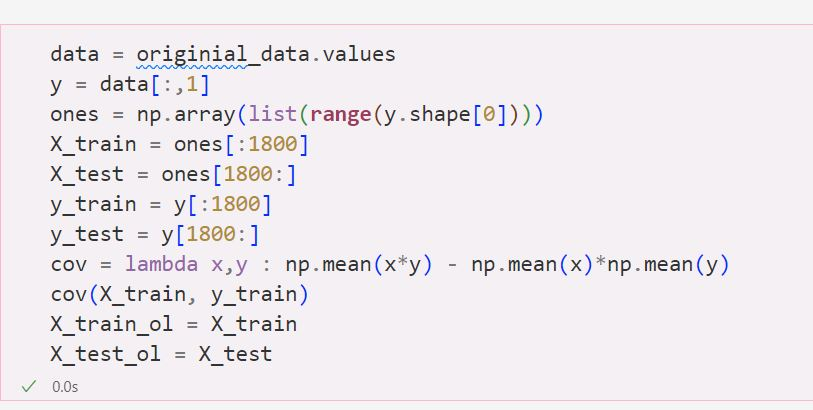
\includegraphics[width=12cm]{homework_code/homework_11/immages/4a1.JPG}
        \item 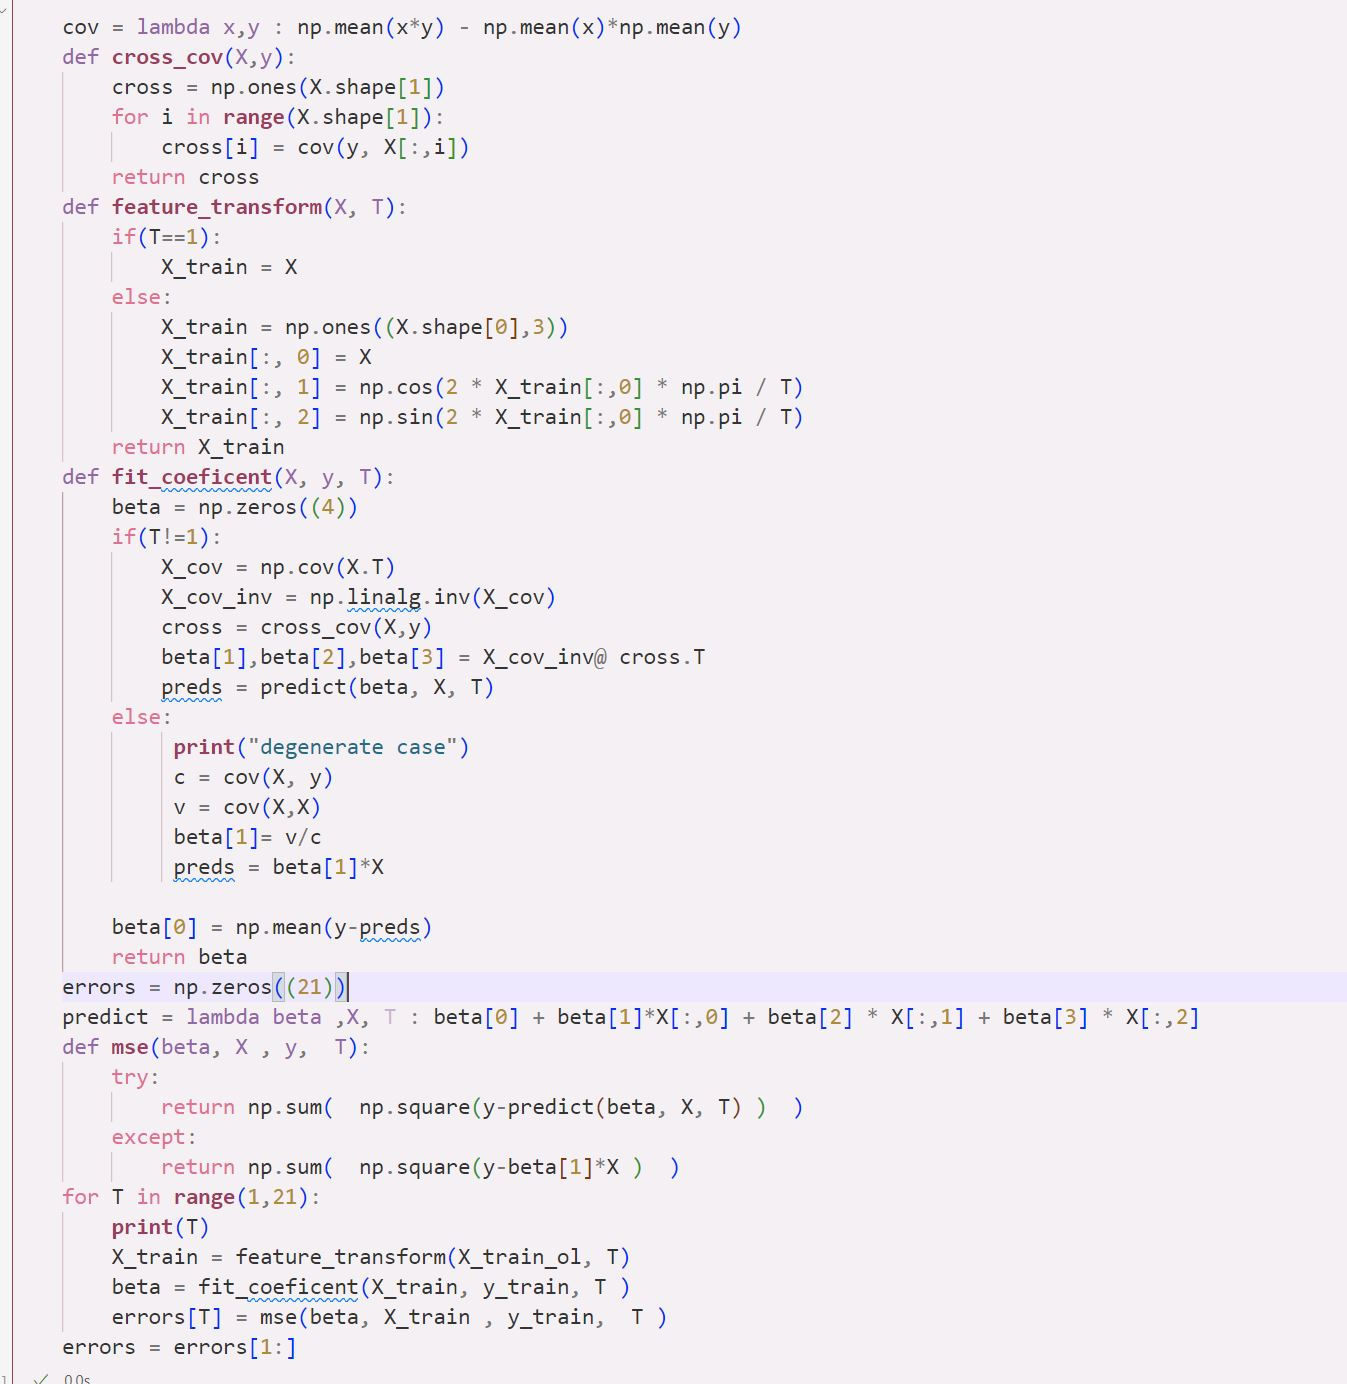
\includegraphics[width=12cm]{homework_code/homework_11/immages/4a2.JPG}
    \end{itemize}
  \item Produce two plots comparing the actual maximum temperatures with
    the ones predicted by your model for $T:=T^{\ast}$; one for the training set and one for the test set. 

    \begin{itemize}
        \item 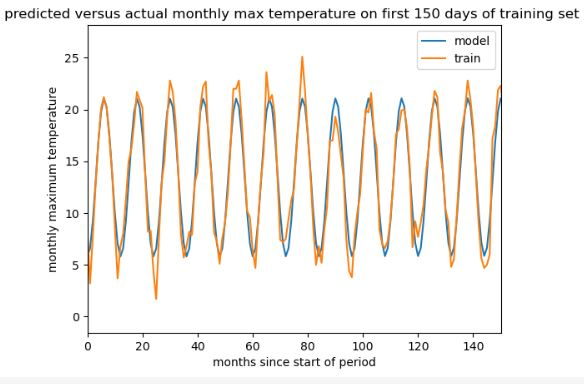
\includegraphics[width=12cm]{homework_code/homework_11/immages/4c1.JPG}
        \item 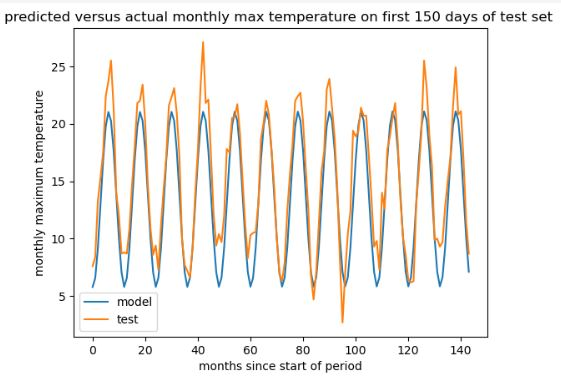
\includegraphics[width=12cm]{homework_code/homework_11/immages/4c2.JPG}

    
        \item 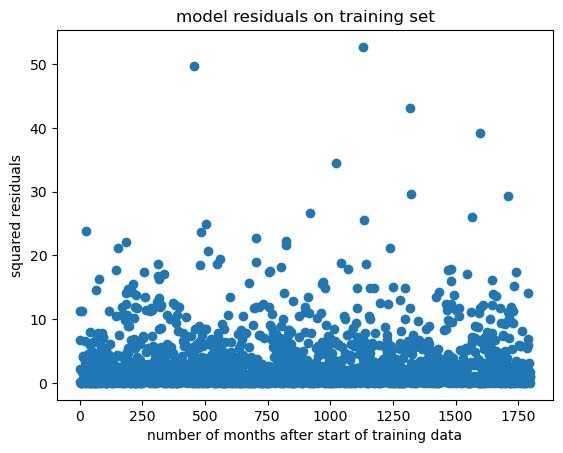
\includegraphics[width=12cm]{homework_code/homework_11/immages/4c1.png}
        \item 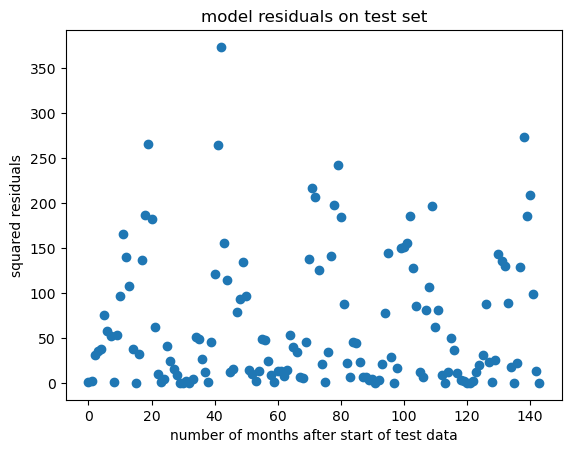
\includegraphics[width=12cm]{homework_code/homework_11/immages/4c2.png}
    \end{itemize}
% \item Fit the modified model  
%   \begin{align}
%  y[t] = a + bt + d \sin(2\pi t/T^{\ast})
%  \end{align}
%and plot the fit to the training data as in the previous question. Explain why it is better to also include a cosine term in the model.
   \item Provide an intuitive interpretation of the coefficients $a$, $b$, $c$ and $d$, and the corresponding features. According to your model, are temperatures rising in Oxford? By how much?
   \begin{itemize}
     \color{blue}
       \item a is the average temperature over the training set, ie our intercept 
       \item b is the linear overall increase in temperature over the training period 
       \item c and d model seasonality, they both have a period of 12 (so 1 year) but they are off cycle so in some period they amplify one another modeling more hot months, in some cases cancel one another modding more temperate months, and in some cases they negatively amplify one another modeling colder months
       \item my b value is 0.00043 so yeah temperatures are rising by around that number of Celsius per year according to my model
       \item we can see by plotting the the predictions for our model, we are effectively fitting 12 separate models one for each month, and all of them have positive slopes with time since start of training set
       \item 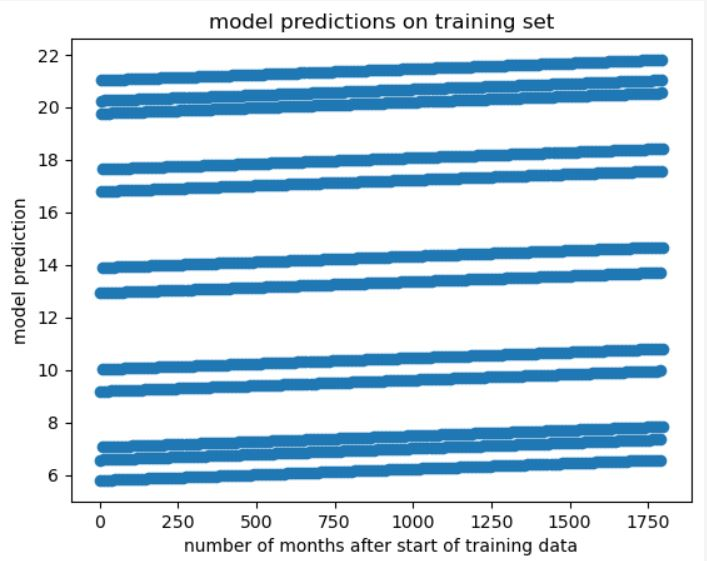
\includegraphics[width=15cm]{homework_code/homework_11/immages/4d.JPG}
   \end{itemize}
  \end{enumerate}

\end{enumerate}
 
\end{document}
